\StartOf{Lecture 11}

\Today{(0) Noise (Notes from Lecture 10); (1) $N$-dim Bayesian Detection Theory}

\announcements{
\begin{itemize}
\item Reading: Today: Rice 6.1, 6.2, Wed: No new reading
\item Project 3 due today at 11:59pm
\item HW 5 due Wed. I will post solutions Thu at midnight so that you can study. 
\item Exam 1 is Mar 2 (one week from today) in class. Exam 1 study material is on Canvas under Pages: View All Pages: Exam 1 Practice.  
\end{itemize}
}

\section{$M$-ary Detection Theory in $N$-dimensional signal space}

We are going to start to talk about QAM, PSK, and FSK, modulations with two dimensional signal vectors. We also consider in this course modulations with higher dimensional signal vectors.  We have developed $M$-ary detection theory for 1-D signal vectors, and now we will extend that to $N$-dimensional signal vectors.

Setup:
\begin{itemize}
 \item Transmit: one of $M$ possible symbols, $\mba_0, \ldots, \mba_{M-1}$.  These vectors are length $N$.
 \item Receive: the symbol plus noise:
\begin{eqnarray}
  H_0: && \mbX = \mba_0 + \mbn \nonumber \\
  \cdots && \cdots \nonumber \\
  H_{M-1}: && \mbX = \mba_{M-1} + \mbn \nonumber
\end{eqnarray}
 \item Assume: $\mbn$ is multivariate Gaussian, each component $n_i$ is independent with zero mean and variance $\sigma_N^2 = N_0/2$.
 \item Assume: Symbols are equally likely.
 \item Question: What are the optimal decision regions?
\end{itemize}

When symbols are equally likely, the optimal decision turns out to be given by the maximum likelihood receiver,
\begin{equation} \label{E:NDimML}
  \hat{i} = \argmax{i} \log f_{\mbX|H_i}(\mbx|H_i)
\end{equation}
Here,
\[
 f_{\mbX|H_i}(\mbx|H_i) = \frac{1}{\sqrt{(2\pi)^{N} \mbox{det}(C_\mbX)} } \exp \left[ -\frac{1}{2}(\mbx-\mba_i)^T  C_\mbX^{-1}
  (\mbx-\mba_i) \right].
\]
But as we derived earlier, the elements of vector $\mbx$ are uncorrelated and each have the same variance $\sigma_N^2$.  This means that 
\[
 f_{\mbX|H_i}(\mbx|H_i) = \frac{1}{(2\pi\sigma_N^2)^{N/2} } \exp \left[ - \sum_{i=0}^{N-1} \frac{(x_k - a_{i,k} )^2 }{2\sigma_N^2} \right]
\]
or
\[
 f_{\mbX|H_i}(\mbx|H_i) = \frac{1}{(2\pi\sigma_N^2)^{N/2} } \exp \left[ - \frac{\|\mbx - \mba_{i}\|^2 }{2\sigma_N^2} \right]
\]
So when we want to solve (\ref{E:NDimML}) we can simplify quickly to:
\begin{eqnarray}
   \hat{i} &=& \argmax{i} \left\{ \log \frac{1}{(2\pi\sigma_N^2)^{N/2} }  -\frac{\|\mbx - \mba_i \|^2 }{2\sigma_N^2} \right\}
   \nnn
   \hat{i} &=& \argmax{i} - \frac{\|\mbx - \mba_i \|^2 }{2\sigma_N^2}
   \nnn
   \hat{i} &=& \argmin{i} \|\mbx - \mba_i \|^2 
   \nnn
   \hat{i} &=& \argmin{i} \|\mbx - \mba_i \|
\end{eqnarray}
Again:  Just find the $\mba_i$ in the signal space diagram which is
closest to $\mbx$.

\subsection{Pairwise Comparisons}

When is $\mbx$ closer to $\mba_i$ than to $\mba_j$ for some other
signal space point $j$? Solution: \textbf{The two decision regions
are separated by a straight line} (Note: replace ``line'' with plane
in 3-D, or subspace in $N$-D).  To find this line:
\begin{enumerate}
  \item Draw a line segment connecting $\mba_i$ and $\mba_j$.
  \item Draw a point in the middle of that line segment.
  \item Draw the perpendicular bisector of the line segment through
  that point.
\end{enumerate}

\Example{ Derive a formula for the dividing line (dividing plane when $N>2$) between $\mba_i$ and $\mba_j$ for $j\neq i$ when symbols are equally likely.}

\Solution{
 Try to find the locus of points $\mbx$ which satisfy the equality of distances between the two symbol points:
\[
  \| \mbx - \mba_i \|^2 = \| \mbx - \mba_j \|^2
\]
You can do this by using the inner product to represent the
magnitude squared operator:
\[
  (\mbx - \mba_i)^T(\mbx - \mba_i) =(\mbx - \mba_j)^T(\mbx - \mba_j)
\]
Then use FOIL (multiply out), cancel, and reorganize to find a
linear equation in terms of $\mbx$.  This is left as an exercise.}



\subsection{Decision Regions}
Each pairwise comparison results in a linear division of space (a half-space).  The
combined decision region, the intersection of all of these of half-spaces, $R_i$, is the space which in which all conditions are satisfied.  This intersection space is where $\mba_i$ is the closest symbol out of all of the $M$ symbols.

A diagram of all of the decision regions is called a Voronoi diagram.

\Example{Optimal Decision Regions} 

We will do an activity in class to draw the decision regions for Bayesian detection for a 2D constellation diagram.  See Figure \ref{F:DetectionRegionsExample} for two randomly generated constellations with $M=5$.

\begin{figure}[htbp]
  \centerline{(a) 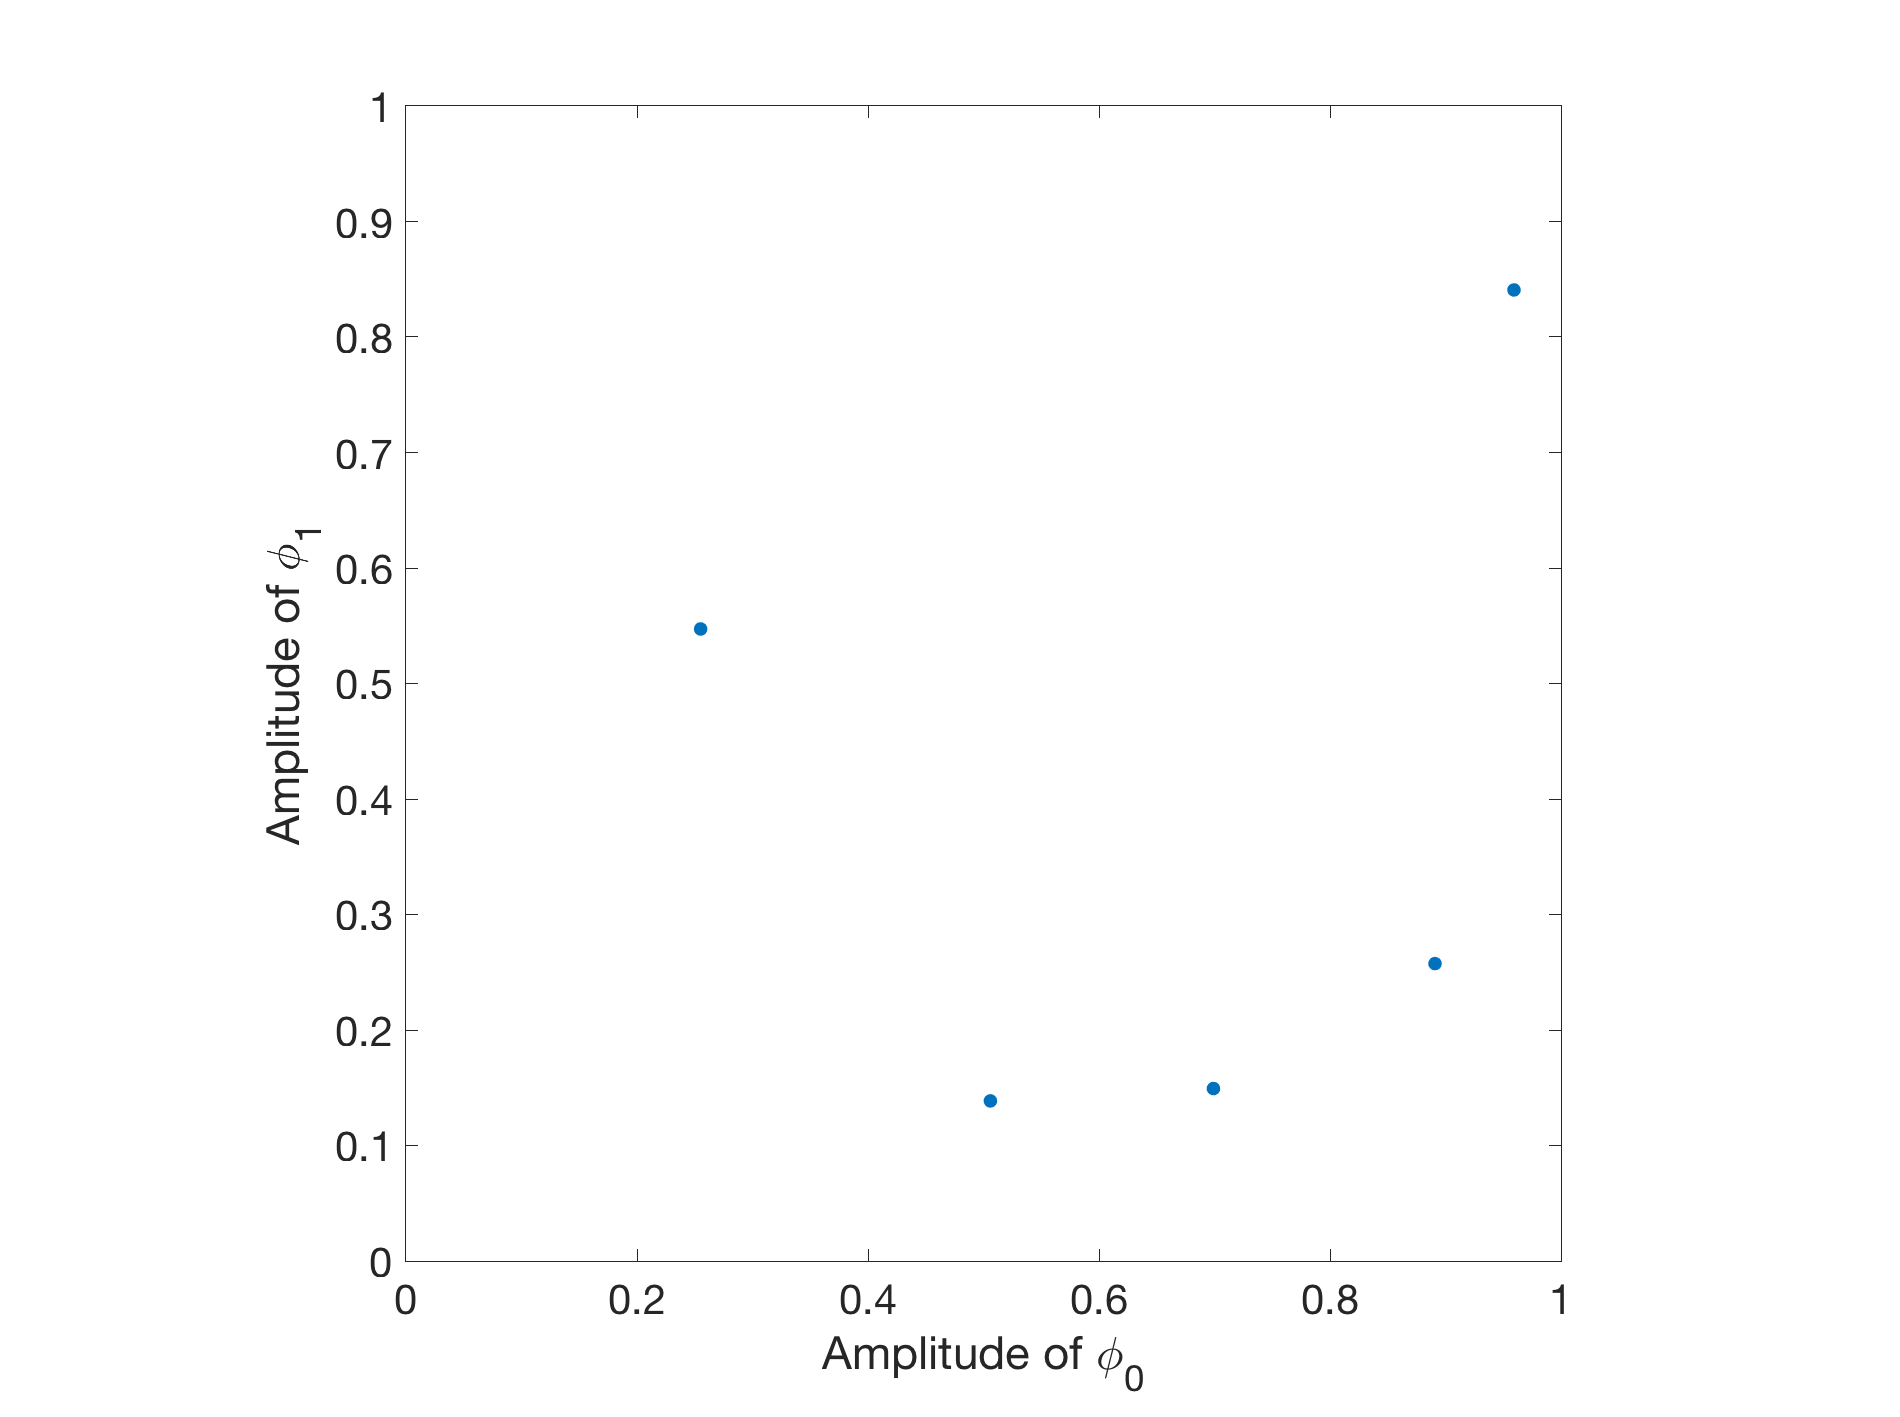
\includegraphics[width=0.9\textwidth]{../images/ExampleVoronoiDiagram_1.png}}
\centerline{  (b) 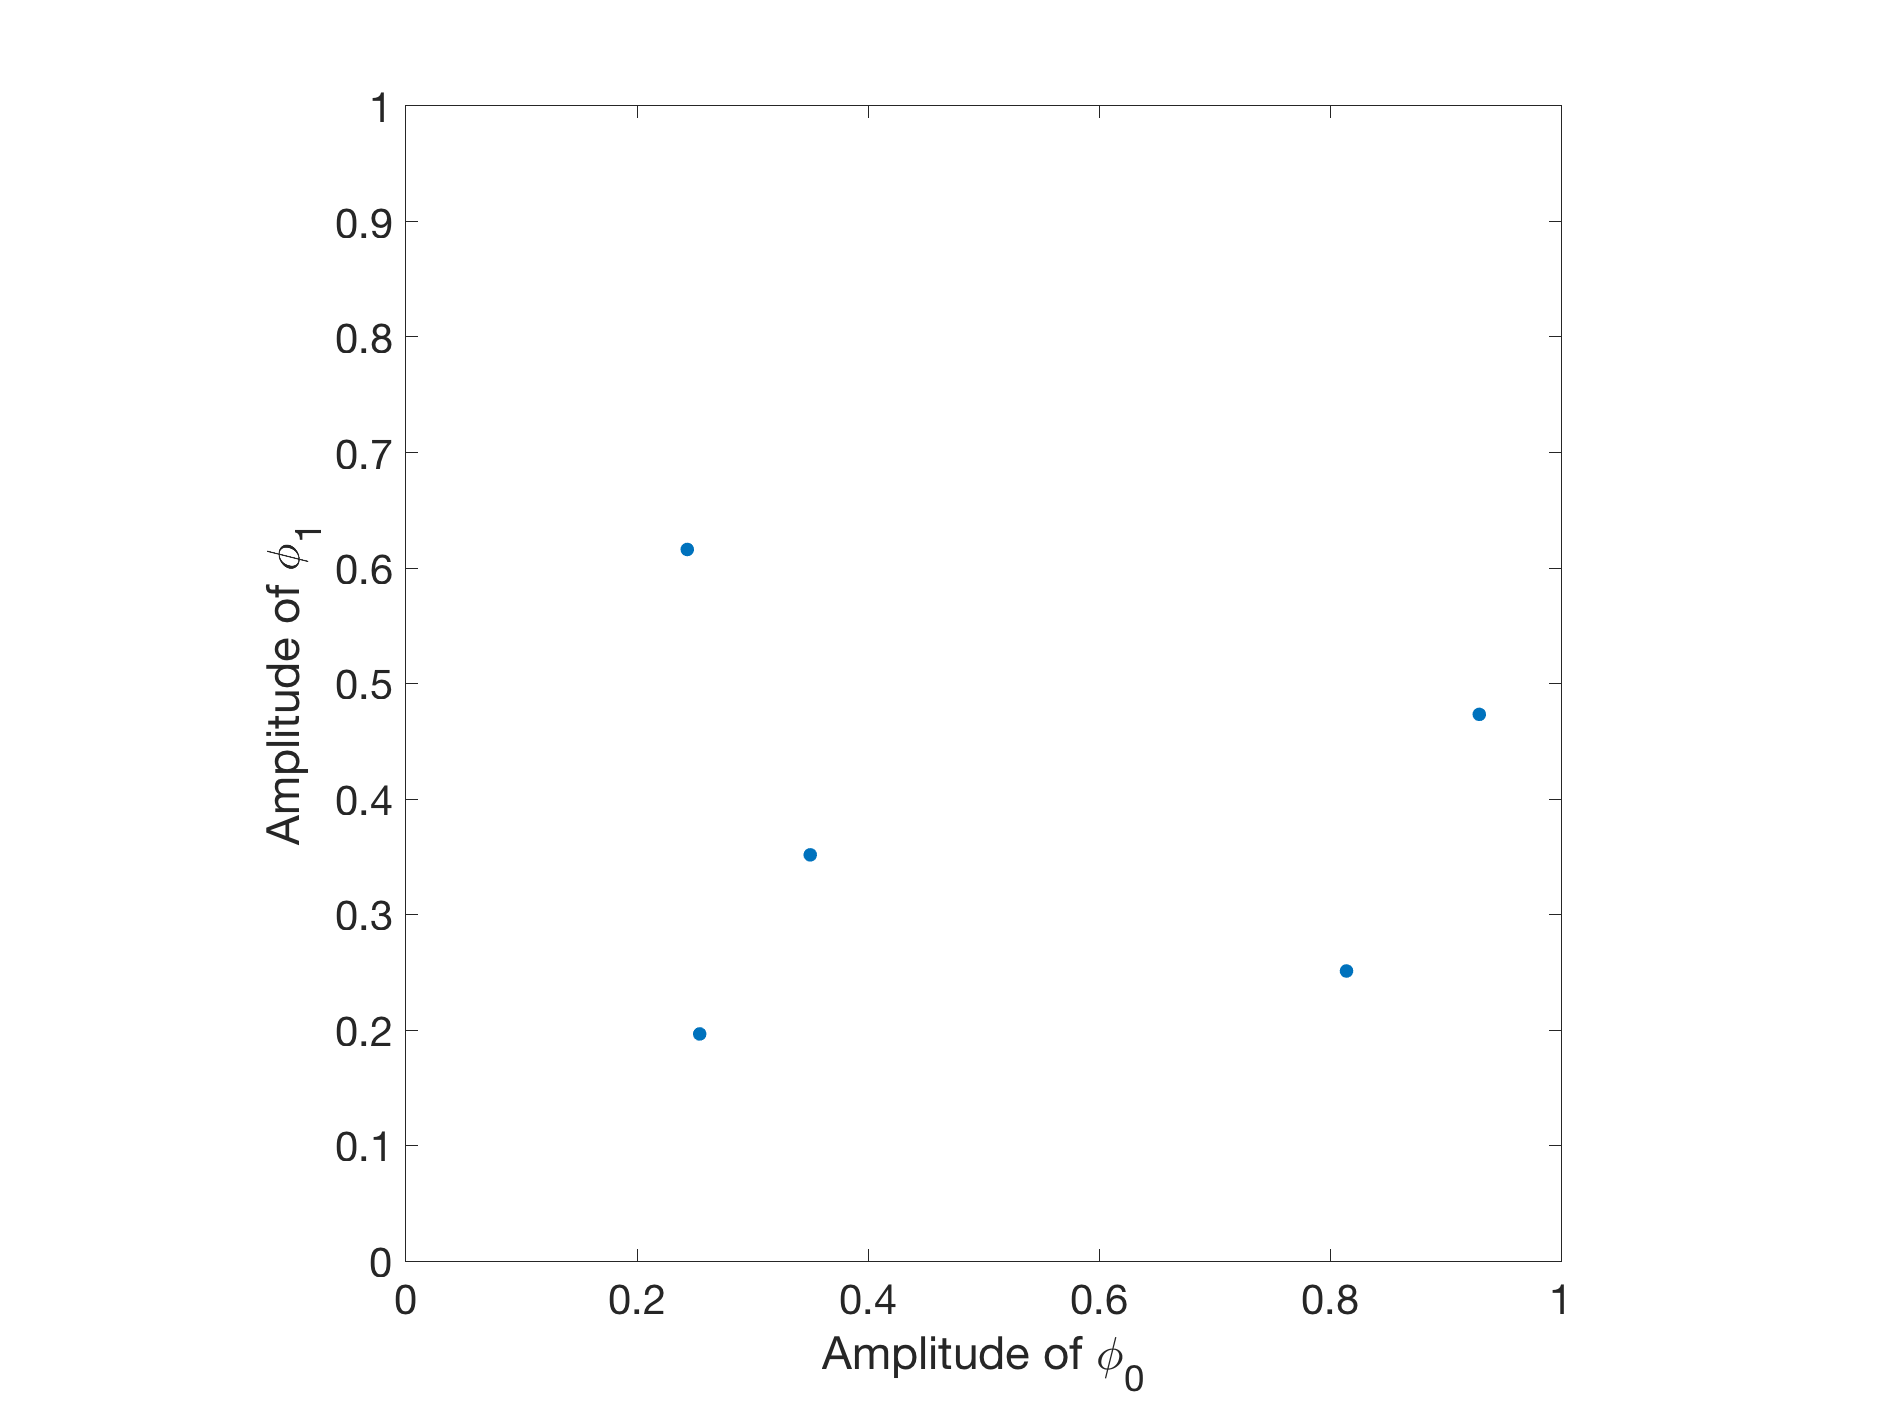
\includegraphics[width=0.9\textwidth]{../images/ExampleVoronoiDiagram.png}}
  \caption{Example signal space diagrams.  Draw the optimal decision regions.}
  \label{F:DetectionRegionsExample}
\end{figure}



\subsection{Symbol Distances}

We mentioned, when talking about signal space diagrams, a distance between vectors,
\[
 d_{i,j} = \| \mba_i - \mba_j \| = \left[ \sum_{k=1}^M (a_{i,k} -
 a_{j,k})^2 \right]^{1/2}
\]
In general we will start to use these distances quite often in the analysis of a modulation method.
